% \section{Data}
\label{sec:data}

Web-scale training data has proven transformative for multi-task and multi-lingual speech systems, delivering substantial performance improvements. However, the scale that enables these gains often comes with quality trade-offs that require careful management. For Canary-1B-v2 and Parakeet-TDT-0.6B-v3, we addressed the data problem from multiple complementary perspectives: task and language balancing, optimal mixing of pseudo-labeled and human-annotated data, and careful curation strategies to maximize data utility while mitigating quality concerns. 

In this section, we present all the datasets that comprise our 1.7M hours of training data used to train both models, provide insights into data composition and future balancing decisions, and detail the evaluation datasets used to assess model performance.


\subsection{Training Data Curation and Sources }
\label{sec:data-training-data}

The training data of \emph{Canary-1B-v2} is heavily based on Granary multilingual and multitask dataset \cite{granary} which is a super set of three main corpora: MOSEL\cite{mosel}, YTC\cite{ytc}, and YODAS\cite{yodas}, comprising around ~0.7 million hours of ASR speech data samples in 25 supported languages, which is pseudo-labeled and translated to other languages for AST tasks with Granary pipeline. Its multi-task speech data components, proven quality of the data processing pipeline, and broad language coverage made it possible to train a model of this scale and scope. However, because much of the data was pseudo-labeled, we also needed to mitigate potential issues that could arise from the limited amount of human-labeled data.

To address this challenge, we augmented Granary with 227,000 hours of high-quality human-labeled data from NeMo ASR Set 3.0, covering all three tasks (ASR, AST X→En, and En→X) across all 25 languages. While representing only 13\% of our total training dataset, NeMo ASR Set provides invaluable human-annotated data sourced from proven quality datasets including AMI~\cite{ami}, FLEURS~\cite{fleurs}, Common Voice~\cite{commonvoice:2020}, Multilingual LibriSpeech (MLS)~\cite{MLS}, and language-specific datasets such as Golos~\cite{golos} for Russian. 


Another crucial addition to the Granary dataset was a supplementary dataset specifically for the En→X translation task, since Granary originally provided data only for ASR and X→En tasks. This supplementary mono-task dataset was constructed by sampling a subset of the Granary English corpus and generating translations into multiple target languages using the methodology described in \cite{granary}. In total, it comprised around 480,000 hours of English-to-non-English audio–transcription pairs.

Figure~\ref{fig:data-dist} summarizes the distribution of tasks across corpora in our training data. As can be observed, there is a task imbalance present in the training set, where ASR and En→X tasks dominate the dataset, while X→En translation data is comparatively limited. This is a common phenomenon in multi-task training setups, for which we have applied mitigating methods described in Section~\ref{sec:training}.

\begin{figure}[htbp]
  \centering
  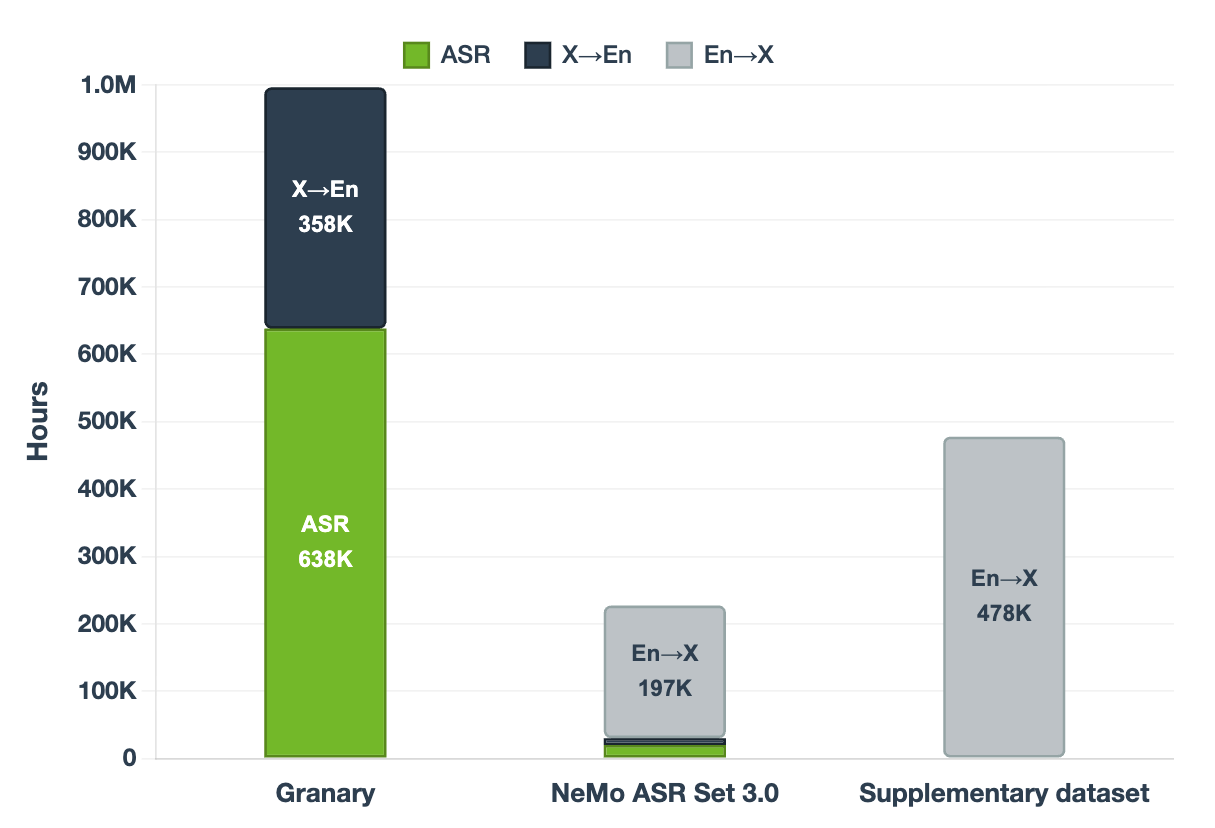
\includegraphics[width=0.6\linewidth]{images/data_by_corpus_and_tasks.png}
  \caption{Overview of participating corpora in the training set with within-corpus task divisions.}
  \label{fig:data-dist}
\end{figure}

For our second model, \emph{Parakeet-TDT-0.6B-v3}, we trained exclusively on the ASR subset of the \emph{Canary-1B-v2} training set (\(\sim\)660,000 hours across the same 25 languages).


\subsection{Non-speech Data for Robustness}

To enhance model robustness against hallucinations, particularly those potentially inherited from Whisper-based pseudo-labeling, we incorporated 36,000 hours of non-speech audio into our training dataset. These samples, extracted during Granary pipeline filtration steps\footnote{\url{https://github.com/NVIDIA/NeMo-speech-data-processor/tree/main/dataset_configs/multilingual/granary}}, are paired with empty string targets to teach the model when not to generate transcriptions.

We randomly assigned source-target language pairs to non-speech samples, creating coverage across all possible task combinations (X→X, En→X, and X→En). This approach ensures the model learns to detect and appropriately handle non-speech content regardless of the specified language pair.

With this final addition, we have around 1.7M hours of combined ASR and AST data. For a more detailed overview of the training data decomposition, refer to Appendix~\ref{app:training_data_overview}.

\subsection{Language Coverage and Imbalance Analysis}
\label{sec:lang-coverage-imbalance}

Our training dataset encompasses all 25 target European languages, with Granary serving as the primary source for low-resource languages such as Latvian (lv), Maltese (mt), and Lithuanian (lt). Through VoxPopuli~\cite{voxpopuli} from MOSEL, we successfully gathered sufficient training material for these languages and generated corresponding X→En translation pairs leveraging Granary pipeline.

English naturally dominates the dataset, comprising approximately 285,000 hours (~40\%) of ASR data. Given English's central role across all three tasks (ASR, X→En, En→X), this dominance supports building a solid foundational knowledge base during pretraining. 

Figure~\ref{fig:language-distribution} presents the training hours distribution for our 24 non-English target languages, revealing important patterns in data availability across tasks. Language imbalance mitigation strategies, including approaches to address English dominance, are detailed in Sections ~\ref{sec:lang-corpora-balancing} and ~\ref{sec:fine-tuning}.

\begin{figure}[htbp]
  \centering
  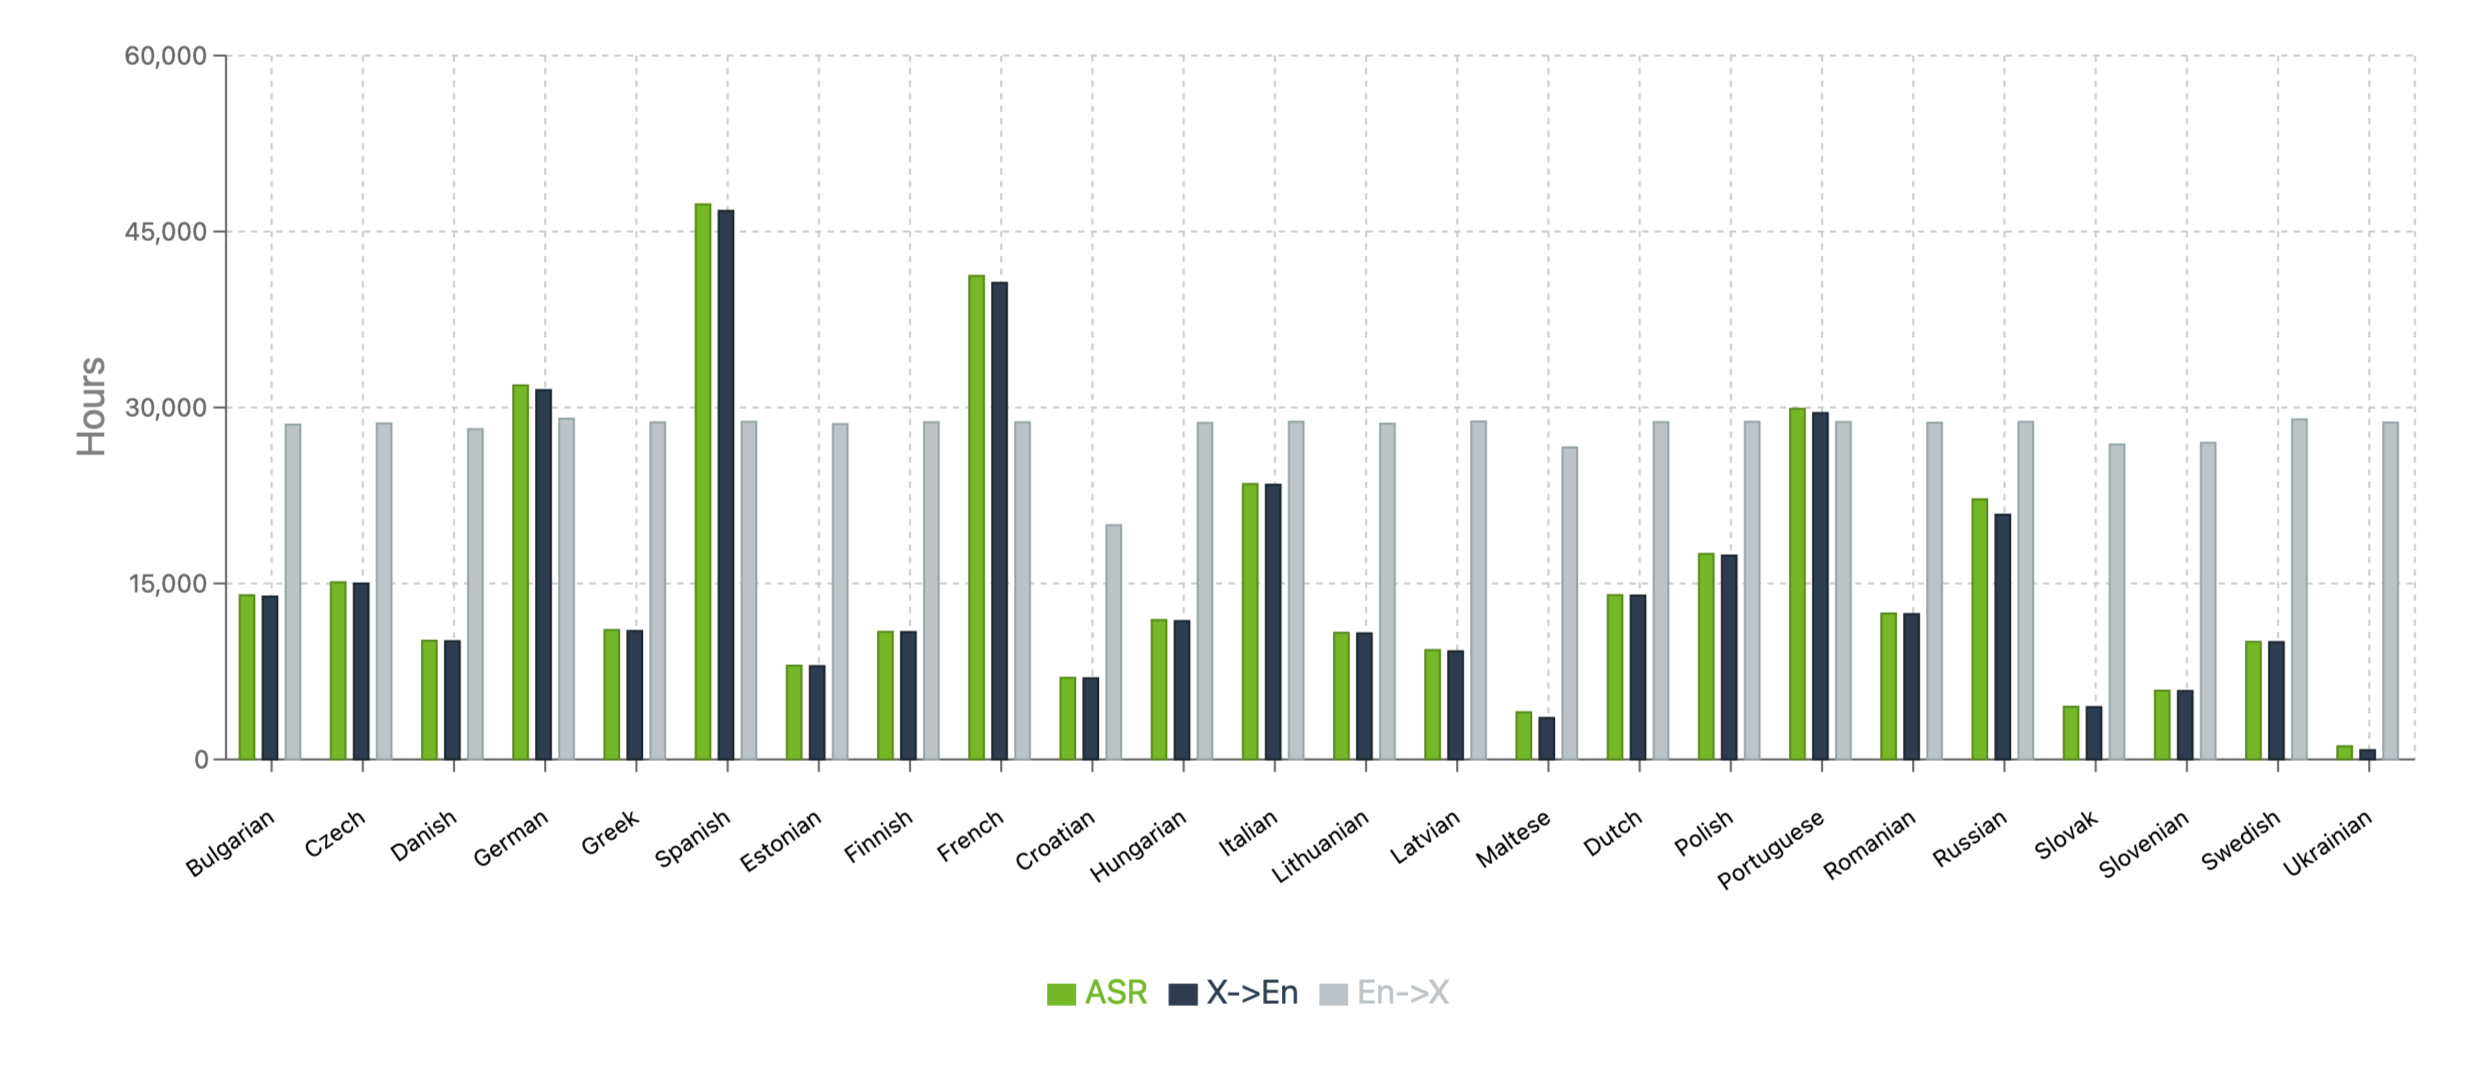
\includegraphics[width=0.95\linewidth]{images/langs_and_tasks.png}
  \caption{Language (non-English) Training Hours Distribution by Task.}
  \label{fig:language-distribution}
\end{figure}

As observed in the Figure~\ref{fig:language-distribution}, the En→X translation direction exhibits relatively uniform data distribution across languages, with values consistently ranging between 20,000-29,000 hours. The primary divergence emerges in ASR and X→En translation tasks, where low-resource languages such as Ukrainian (790 hours), Maltese, Estonian, and Slovak contrast sharply with high-resource languages including Spanish, French, German, Italian, Portuguese, and Russian, which dominate with significantly higher training hours. Given this pronounced imbalance and the fact that VoxPopuli data from the Granary corpus serves as the primary ASR source, we further analyze the ASR data source composition in the subsequent Figure~\ref{fig:language-corpus}.

When examining the relative volumes of Granary sub-corpora and NeMo ASR Set 3.0 in the ASR data for each language under study, a clear trend emerges. Except for high-resource, well-represented languages such as German, Spanish, French, Italian, Portuguese, and Russian, the Voxpopuli subset of the Granary corpus dominates, comprising over 95\% of the data for most languages. This dominance of Voxpopuli creates two primary issues for these languages: (a) Voxpopuli recordings originate from EU parliament sessions, where the language register differs significantly from everyday conversational speech, leading to narrow-domain data dominance; and (b) Voxpopuli consists primarily of 30-second audio segments, which limits the acoustic and linguistic diversity available for languages dominated by this corpus. We reserve Voxpopuli audio resegmentation for future work. Despite these limitations, we cannot eliminate Voxpopuli entirely, as doing so would remove 15 unique languages from our 25-language set, contradicting our objective of supporting low-resource language inclusion.

\begin{figure}[htbp]
  \centering
  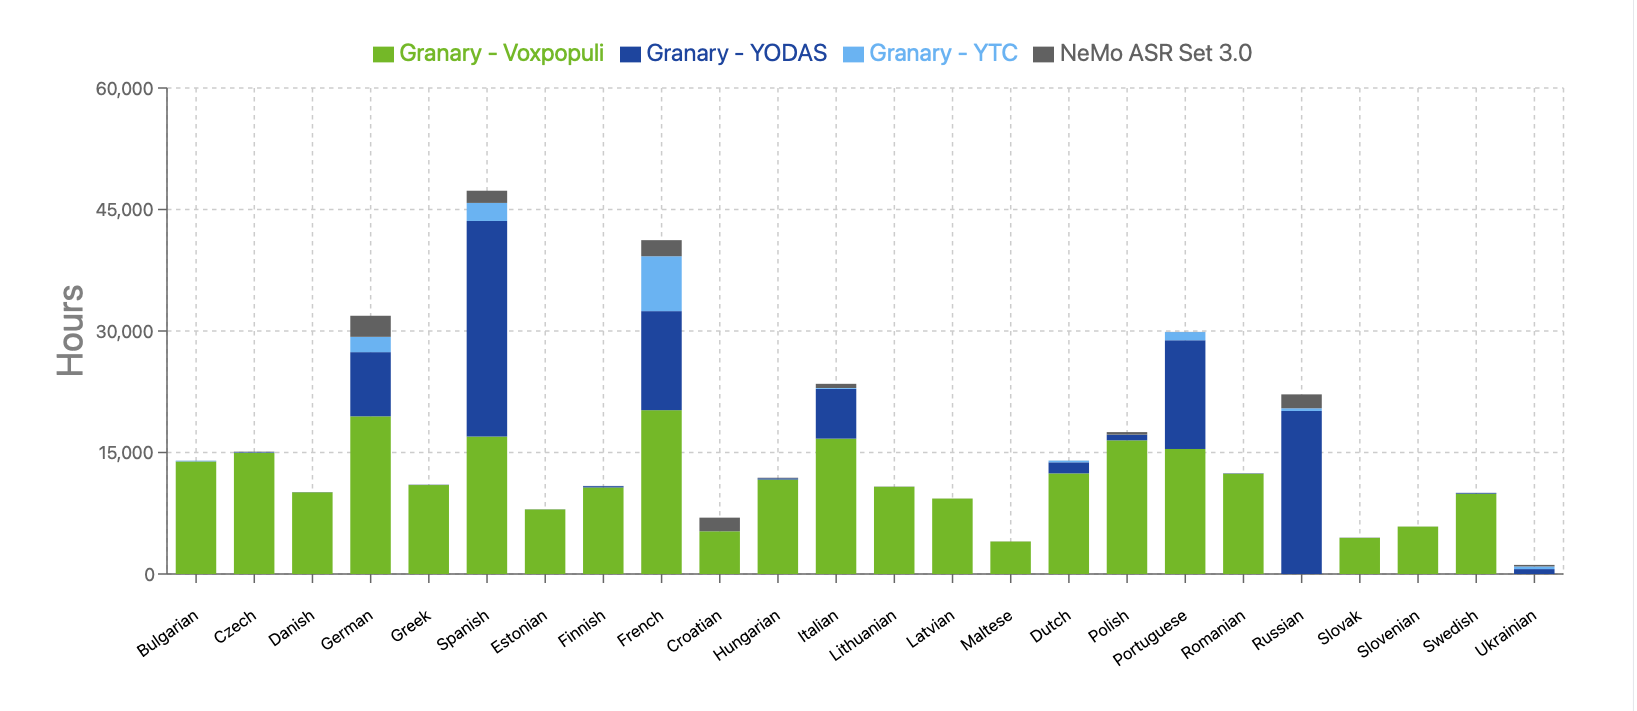
\includegraphics[width=0.95\linewidth]{images/langs_and_corpuses.png}
  \caption{Language (non-English) ASR Data Training Hours Distribution by Corpus.}
  \label{fig:language-corpus}
\end{figure}

For detailed numerical breakdowns of training hours by language, corpus, and task, refer to Appendix~\ref{app:lang_dist}.

\subsubsection{Balancing Languages and Corpora}
\label{sec:lang-corpora-balancing}

Building on the preceding analysis of language and corpora imbalance, we adopt a two-tier sampling policy that (i) balances corpora \emph{within} each language and (ii) balances \emph{across} languages. During pre-training, each direction is treated as a distinct “language” entry (e.g., \texttt{lv}, \texttt{lv--en}, \texttt{en--lv}), so the policy applies uniformly to ASR and AST.  

We followed the general methodology described in \cite{xlsr}, with one key modification. In \cite{xlsr}, the procedure first upsamples languages within a corpus and then balances the different corpora by treating each corpus as a separate language. In contrast, our approach inverts this order: we first perform corpus balancing within each language, and only then apply language balancing across the training corpora. This adjustment ensures that low-resource corpora within a language are not overshadowed before cross-language balancing is applied. Our procedure consists of three steps:

\begin{enumerate}
  \item \textbf{Corpus balancing within language.}  
  For a given language $l$, we first compute unnormalized weights for each corpus $c \in l$:
  \[
  w_c = \left(\frac{n(c)}{N_l}\right)^{\alpha},
  \]
  where $n(c)$ is the number of hours in corpus $c$, $N_l = \sum_{c \in l} n(c)$ is the total number of training hours for language $l$, and $\alpha \in (0,1]$ is a subsampling factor controlling the trade-off between high-resource and low-resource corpora.  
  The normalized distribution over corpora within language $l$ is then
  \[
  p_c = \frac{w_c}{\sum_{c \in l} w_c}, \quad \sum_{c \in l} p_c = 1 .
  \]

  \item \textbf{Language balancing across training corpora.}  
  Next, we compute unnormalized weights for languages:
  \[
  w_l = \left(\frac{n(l)}{N_\text{total}}\right)^{\beta},
  \]
  where $n(l) = \sum_{c \in l} n(c)$ is the total number of hours for language $l$, $N_\text{total} = \sum_l n(l)$ is the global total across all languages, and $\beta \in (0,1]$ is an upsampling factor controlling the degree of balance between high- and low-resource languages.  
  The normalized distribution over languages is then
  \[
  p_l = \frac{w_l}{\sum_{l'} w_{l'}}, \quad \sum_l p_l = 1 .
  \]

  \item \textbf{Final entry distribution.}  
  The final probability of sampling from a corpus $c$ in language $l$ is the product
  \[
  p_{c,l} = p_l \cdot p_c .
  \]
\end{enumerate}

In practice, we set both the corpus-level subsampling factor and the language-level upsampling factor to $\alpha = 0.5$ and $\beta = 0.5$, respectively. Having computed these distributions, we leveraged the Lhotse multi-functional library \cite{lhotse} to form batches according to $p_{c,l}$. This ensured diverse sampling at each step. Our analysis showed that, despite the inherent imbalance across languages and tasks, the upsampling procedure consistently produced batches containing at least 14 distinct language pairs.

\subsection{Evaluation Benchmarks}
\label{sec:evaluation-benchmarks}

Having established our training data composition, we now describe the evaluation benchmarks used to assess model performance across tasks and languages.

As canary-1b-v2 is multi-task model, it required comprehensive multi-task evaluation sets for assessment. For this purpose, we primarily used the FLEURS dataset, which included all 25 languages of our focus. In addition to the FLEURS dataset, we also utilized CoVoST\cite{covost2} and Multilingual LibriSpeech (MLS) data. The latter two datasets did not represent all 25 languages, but rather covered a subset of them. See Table~\ref{tab:evaluation-datasets} for complete details on the evaluation datasets and their language coverage.

\begin{table}[ht]
\centering
\small
\setlength{\tabcolsep}{6pt}
\setlength{\abovecaptionskip}{10pt} % add space between table and caption
\renewcommand{\arraystretch}{1.15}
\begin{tabular}{l|ccc|cc|cc}
\toprule
 & \multicolumn{3}{c|}{\textbf{ASR}} & \multicolumn{2}{c|}{\textbf{X$\to$En}} & \multicolumn{2}{c}{\textbf{En$\to$X}} \\
\textbf{Lang} & Fleurs & MLS & CoVoST2 & Fleurs & CoVoST2 & Fleurs & CoVoST2 \\
\midrule
bg & \checkmark & -- & -- & \checkmark & -- & \checkmark & -- \\
cs & \checkmark & -- & -- & \checkmark & -- & \checkmark & -- \\
da & \checkmark & -- & -- & \checkmark & -- & \checkmark & -- \\
de & \checkmark & -- & \checkmark & \checkmark & \checkmark & \checkmark & \checkmark \\
el & \checkmark & -- & -- & \checkmark & -- & \checkmark & -- \\
en & \checkmark & -- & \checkmark & -- & -- & -- & -- \\
es & \checkmark & \checkmark & \checkmark & \checkmark & \checkmark & \checkmark & -- \\
et & \checkmark & -- & \checkmark & \checkmark & \checkmark & \checkmark & \checkmark \\
fi & \checkmark & -- & -- & \checkmark & -- & \checkmark & -- \\
fr & \checkmark & \checkmark & \checkmark & \checkmark & \checkmark & \checkmark & -- \\
hr & \checkmark & -- & -- & \checkmark & -- & \checkmark & -- \\
hu & \checkmark & -- & -- & \checkmark & -- & \checkmark & -- \\
it & \checkmark & \checkmark & \checkmark & \checkmark & \checkmark & \checkmark & -- \\
lt & \checkmark & -- & -- & \checkmark & -- & \checkmark & -- \\
lv & \checkmark & -- & \checkmark & \checkmark & \checkmark & \checkmark & \checkmark \\
mt & \checkmark & -- & -- & \checkmark & -- & \checkmark & -- \\
nl & \checkmark & \checkmark & \checkmark & \checkmark & \checkmark & \checkmark & -- \\
pl & \checkmark & \checkmark & -- & \checkmark & -- & \checkmark & -- \\
pt & \checkmark & \checkmark & \checkmark & \checkmark & \checkmark & \checkmark & -- \\
ro & \checkmark & -- & -- & \checkmark & -- & \checkmark & -- \\
ru & \checkmark & -- & \checkmark & \checkmark & \checkmark & \checkmark & -- \\
sk & \checkmark & -- & -- & \checkmark & -- & \checkmark & -- \\
sl & \checkmark & -- & \checkmark & \checkmark & \checkmark & \checkmark & \checkmark \\
sv & \checkmark & -- & \checkmark & \checkmark & \checkmark & \checkmark & \checkmark \\
uk & \checkmark & -- & \checkmark & \checkmark & -- & \checkmark & -- \\
\bottomrule
\end{tabular}
\caption{Language coverage by task and dataset in evaluation set. A checkmark indicates that language is present in the corresponding dataset for the given task.}
\label{tab:evaluation-datasets}
\end{table}

In addition to these multilingual benchmarks, we evaluated our model on the Hugging Face Open ASR Leaderboard datasets\cite{open-asr-leaderboard} for comprehensive English ASR assessment and competitive benchmarking against other state-of-the-art models.

